\documentclass{article}
\usepackage{graphicx}
\usepackage[normalem]{ulem}
\usepackage[margin=1.5cm]{geometry}
\usepackage{amsmath}

\begin{document}

\title{Laboratory on Net Force: Force Tables}
\author{Prof. Jordan C. Hanson}

\maketitle

\begin{figure}[ht]
\centering
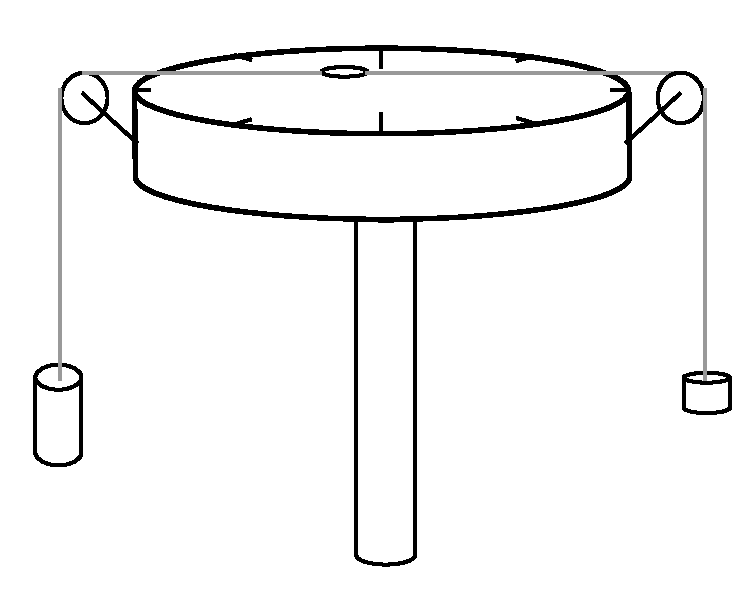
\includegraphics[width=0.2\textwidth]{figures/Table.pdf}
\caption{\label{fig:table} The force table setup includes a wheel with angles, strings and pulleys, and a central ring.}
\end{figure}

\section{Memory Bank}

\begin{enumerate}
\item The \textit{weight} of a system is the mass times the gravitational constant, $g$.  Written as an equation:
\begin{equation}
\vec{w} = - m g \hat{j}
\end{equation}
When a mass is suspended by a string or rope, the \textit{tension} in the rope balances the weight.
\end{enumerate}

\section{Force Table Lab Setup}

Obtain a set of weights, and a force-table, with ring and pulley system.  Make the angle between two of the strings 60 degrees.  Choose two different weights, $m_1$ and $m_2$.  Set $m_1$ on 0 degrees, and set $m_2$ on 60 degrees.  We will determine the mass $m_3$ that keeps the ring stationary if hung at the correct angle.

\section{Details of the Measurement}

\begin{enumerate}
\item Treating the tension $\vec{T}_1$ (with $m_1$) and the tension $\vec{T}_2$ (with $m_2$) as vectors, break them into components:
\\ \\
\underline{$T_{1,x}=$ \hspace{1cm} (N)} \hspace{0.5cm} \underline{$T_{1,y}=$ \hspace{1cm} (N)} \hspace{1cm} \underline{$T_{2,x}=$ \hspace{1cm} (N)} \hspace{0.5cm} \underline{$T_{2,y}=$ \hspace{1cm} (N)}
\item Determine $\vec{T}_3$ such that $\vec{F}_{\rm Net} = 0$:
\begin{table}[hb]
\centering
\begin{tabular}{| c | c | c |}
\hline
Vector & x-component (N) & y-component (N) \\ \hline
$\vec{T}_1$ & & \\ \hline
$\vec{T}_2$ & & \\ \hline
$\vec{T}_3$ & & \\ \hline
$\vec{F}_{\rm Net}$ & & \\ \hline
\end{tabular}
\caption{\label{tab:data} Break the vectors into components here.}
\end{table}
\item Knowing that $|\vec{T}_3| = m_3 g$, solve for $m_3$ by finding $|T_{3}|$.  Knowing the components of $\vec{T}_3$, solve for the angle it makes with the x-axis.  Arrange $\vec{T}_3$ on the table.  \textbf{Is the ring stationary?}
\end{enumerate}

\end{document}
